% Морфологические операции. Эрозия, дилатация, замыкание и размыкание: что это и для чего могут быть использованы.

\begin{definition}{Морфологическая операция}
    Пусть дано изображение $I$ в оттенках серого и некоторый структурный элемент $S$ -- небольшое черно-белое изображение, на котором выделена некоторая начальная точка (как правило, в центре изображения). Тогда под \textbf{морфологической операцией} понимается преобразование $I$ в выходное изображение $B$ такого же размера, где значение каждой точки $B_{ij}$ определяется по следующему правилу:
    \begin{enumerate}
    \item
        Структурный элемент совмещается с исходным изображением так, чтобы точка $I_{ij}$ совпала с начальной точкой $S$;
    \item
        Из исходного изображения выделяется набор точек, на которые накладываются белые точки структурного элемента;
    \item
        $B_{ij}$ определяется как некоторая заданная функция от значений выделенного набора точек (например, среднее, максимум/минимум)
    \end{enumerate}
\end{definition}

Выделяют следующие стандартные операции:

\paragraph{Эрозия.}

В случае эрозии заданная функция -- это минимум, поэтому эта операция также называется <<оконным минимумом>>. Эта операция полезна для удаления небольших объектов, в том числе шумов (в предположении, что объекты светлее фона), однако она затирает части объектов вблизи границы. Обозначение: $B = I \ominus S$.

\paragraph{Дилатация.}

Заданная функция -- максимум. В случае, если исходное изображение -- бинарное, эта операция эквивалентна смазу, при котором в качестве point spread function используется $S$. Обозначение: $B = I \oplus S$.

\paragraph{Замыкание (closing).}

Замыкание -- операция, которая задается как комбинация дилатации и эрозии (в таком порядке): $B = (I \oplus S) \ominus S$.

\paragraph{Размыкание (opening).}

Размыкание -- операция, которая задается как комбинация эрозии и дилатации (в таком порядке): $B = (I \ominus S) \oplus S$. Эта операция используется для выделения темного фона: сначала при помощи эрозии удаляются шумы и маленькие объекты, а затем при помощи дилатации восстанавливаются удаленные границы. При помощи вычитания размыкания из исходного изображения можно получить объекты, очищенные от фона. Это полезно, например, для выделения текста на изображении с неравномерным освещением, что можно видеть на изображении \ref{opening_demo}.

\begin{figure}[!h]
    \centering
    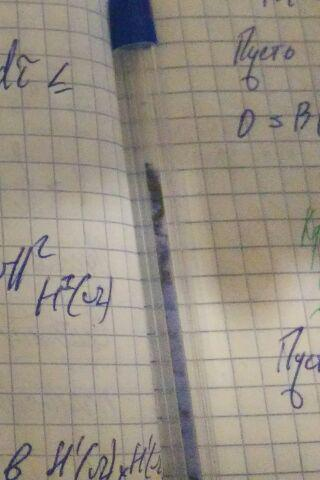
\includegraphics[width=0.3\linewidth]{2_orig}
    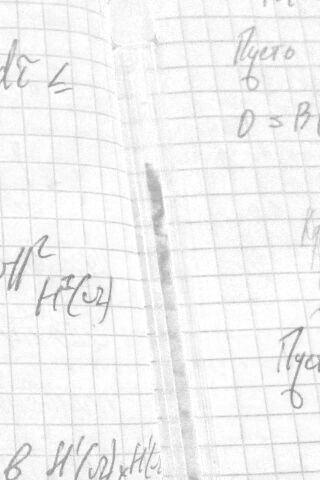
\includegraphics[width=0.3\linewidth]{2_diff}
    \caption{Исходное изображение (слева) и разность между исходным изображением и размыканием (справа).}
    \label{opening_demo}
\end{figure}

